\documentclass[a4paper]{article}
\pdfoutput=1
\usepackage[utf8]{inputenc}
\usepackage{jheppub}
\usepackage{overpic}
\usepackage{subcaption}
\usepackage{fancybox}
\usepackage{float}
\usepackage{amsfonts}
\usepackage{amsmath}
\usepackage{amsbsy}
\usepackage{graphicx}
\usepackage{amssymb}
\usepackage{amsthm}
\usepackage{bm}
\usepackage{comment}
\usepackage{epsfig}
\usepackage{latexsym}
\usepackage{pdflscape}
\usepackage{color}
\usepackage{slashed}
\usepackage{tikz}
\usetikzlibrary{arrows.meta,decorations.markings}

\tikzset{
  mid arrow/.style={
    postaction={
      decorate,
      decoration={
        markings,
        mark=at position 0.5 with {\arrow{Stealth[length=6pt,width=6pt]}}
      }
    }
  }
}

\usepackage{cancel}
\usepackage{xcolor}
\usepackage{braket}
\usepackage{empheq}
\usepackage{graphicx} % Allows including images
\usepackage{tikz-3dplot}
% réglage de la vue 3D : élévation=20°, azimut=110°
\tdplotsetmaincoords{20}{110}
\usetikzlibrary{decorations.pathreplacing,calc}
\usetikzlibrary{decorations.pathmorphing}

\definecolor{blue5}{rgb}{0, 0, 0.66666}
\definecolor{red4}{rgb}{0.8, 0, 0}
\definecolor{navyblue}{rgb}{0, 0.2745, 0.67843}
\definecolor{cornflowerblue}{rgb}{0.388235, 0.6941176, 0.898039}
\definecolor{forestgreen}{rgb}{0.13, 0.55, 0.13}
\usetikzlibrary{decorations.text,decorations.pathmorphing}

%Removes Header------------------------------------
\makeatletter
\def\@fpheader{\relax}
\makeatother



\usepackage{orcidlink}

%\DeclareMathOperator{\tr}{tr}
\DeclareMathOperator{\pf}{pf}
\DeclareMathOperator{\Ai}{Ai}
\DeclareMathOperator{\vol}{vol}
\DeclareMathOperator{\sgn}{sgn}
\DeclareMathOperator{\sn}{sn}
\DeclareMathOperator{\cn}{cn}
\DeclareMathOperator{\dn}{dn}
\DeclareMathOperator{\cd}{cd}
\DeclareMathOperator{\Det}{Det}
\DeclareMathOperator{\sech}{sech}
% \DeclareMathOperator{\tr}{tr}

\newcommand{\beq}{\begin{eqnarray}}
\newcommand{\eeq}{\end{eqnarray}}
\newcommand{\bea}{\begin{eqnarray}}
\newcommand{\eea}{\end{eqnarray}}
\newcommand{\be}{\begin{equation}}
\newcommand{\ee}{\end{equation}}
\newcommand{\bq}{\begin{equation}}
\newcommand{\eq}{\end{equation}}
\newcommand{\unit}{1\!\!1}
\newcommand{\half}{\frac{1}{2}}
\newcommand{\nn}{\nonumber}
\newcommand{\no}{\nonumber}
\def\tb{\tilde{\beta}}
\newcommand{\mpl}{M_{\rm Pl}}
\def\k{\kappa}

\newcommand{\bto}{\bar{\tau}^{\textbf{I}}}
\newcommand{\btt}{\bar{\tau}^{\textbf{II}}}




%%% Other definitions


\def\sp{\;\;\;,\;\;\;}
\def\l{\lambda}
%\def\z{\zeta}
\def\lab{\label}
\def\f{H}
\def\La{\Lambda}
\def\z{\zeta}
\def\t{\tau}
\def\e{\epsilon}
\def\o{\omega}
\def\le{\left}
\def\ri{\right}
\def\y{\psi}
\def\half{\frac12}
\def\q{\theta}
\def\cO{{\cal O}}
\def\m{\mu}
\def\n{\nu}
\def\td{\tilde}
\def\d{\delta}
\def\6{\partial}
\def\de{\partial}
\def\del{\nabla}
\def\ls{\ell_s}
\def\a{\alpha}
\def\b{\beta}
\def\lab{\label}
\def\parl{\parallel}
\def\tom{\tilde{\o}}
\def\dA{\dot{A}}
\def\dh{\dot{h}}
\def\df{\dot{f}}
\def\dX{\dot{X}}
\def\bo{\bar{\o}}
\def\r{x}
\def\bo{b_0}
\def\br{\bar{r}}
\def\dx{\delta X^\parl}
\def\dxy{\delta X^2}
\def\dxz{\delta X^3}
\def\ol{\overline}
\def\GM#1{\textit{[GM: #1]}}
\def\g{\gamma}
\def\s{\sigma}
\def\tr{{\rm Tr}}
\def\eps{\epsilon}
\def\fb{f}
\def\rd{\rm d}
\newcommand{\bom}[1]{\fboxsep2mm\fbox{
           $ \displaystyle{ #1} $}}
           
           \newcommand{\rar}{\rightarrow}
\newcommand{\bb}{\mathbb}
\newcommand{\mc}{\mathcal}
\newcommand{\im}{\mathrm{Im}}
\newcommand{\re}{\mathrm{Re}}
\newcommand{\mi}{\sqrt{|\mathcal{I}_4|}}


\def\lab{\label}
\def\le{\left}
\def\ri{\right}
\def\6{\partial}
\def\eps{\epsilon}


% Color definitions
\newcommand{\red}[1]{{\color{red} #1 \color{black}}}
\newcommand{\blue}[1]{{\color{blue} #1 \color{black}}}
\newcommand{\green}[1]{{\color{green} #1 \color{black}}}
\newcommand{\yellow}[1]{{\color{yellow} #1 \color{black}}}
\newcommand{\purple}[1]{{\color{purple} #1 \color{black}}}


% Comment Abbreviations
\newcommand{\IT}[1]{{\red{IG: #1}}} %Ioannis
\newcommand{\PB}[1]{{\blue{PB: #1}}} % Panos
\newcommand{\OP}[1]{{\green{OP: #1}}} % Olga
\newcommand{\PG}[1]{{\purple{PG: #1}}} % Paul

\title{Comite de Suivi}

\author[a]{Paul Ghiringhelli,}
\affiliation[a]{\href{https://www.cpht.polytechnique.fr/?q=en}{CPHT, CNRS, École polytechnique, Institut Polytechnique de Paris},  91120 Palaiseau, France}

\emailAdd{paul.ghiringhelli@polytechnique.edu}


\begin{document}
\maketitle
\flushbottom


%%%%%%%%%%%%%%%%%%%%%%%%%%%%%%%%%%%%%%%%%%%%%%%%%%%%%%%%%%

\section{Introduction}

The objective of the present report is to provide an overview of the current status of the research projects pursued over the past year. The work I have conducted so far has focused on aspects of quantum cosmology in four dimensions, as well as on well-defined lower-dimensional toy models. Although the tools employed in these two settings are quite different, I believe that they share a common feature: they allow us to sharpen our understanding of the issues and features associated with quantizing a theory of gravity.

In the context of cosmology, the problem of quantizing gravity in Einstein's theory is nicely encapsulated by the Hartle–Hawking proposal for the wavefunction of the universe~\cite{PhysRevD.28.2960}. In 1983, Hartle and Hawking postulated that the wavefunction of the universe should be computed as a path integral over compact geometries in the Euclidean past,
\begin{equation}
\Psi_{\rm N.B} [h_{ij}, \phi_0] = \int ^{g_{ij}|_{\partial \mathcal{M}} = h_{ij}} \rm{D}g \int ^{\phi|_{\partial \mathcal{M}}= \phi_0} \rm{D}\phi \, e^{-\mathcal{S}_{E}[g,\phi]} , .
\end{equation}
Here, $\partial \mathcal{M}$ denotes the boundary of themanifold $\mathcal{M}$, $h_{ij}$ is the induced metric on the boundary, and $\phi_0$ is the value of the matter field there. The path integral is taken over all compact Euclidean geometries with a single boundary on which the induced metric and matter field are respectively $h_{ij}$ and $\phi_0$. Owing to the complexity of such an object, the path integral cannot be computed exactly, and one must resort to a series of truncations and approximations in order to evaluate it.

A well-known result in the context of single-field slow-roll inflation is obtained from the WKB evaluation of the minisuperspace truncation of the path integral. The modulus of the no-boundary instanton wavefunction\footnote{In the context of quantum cosmology, the relevant manifold descrbing the no-boundary instanton is a complex geometry that smoothly interpolates between a Euclidean geometry and a Lorentzian geometry. The Lorentizan evolution gives a multiplicative oscillatory term.} is proportional to 
\begin{equation}
|\Psi_{\rm N.B}[h_{ij}, \phi_0]| \propto \exp\left[+\frac{12\pi^2}{\kappa^2 V(\phi_\star)}\right], \qquad \kappa = 8 \pi G_{N} \,,
\end{equation}
where $\phi_\star$ is the value of the inflaton field at the turning point of the geometry, corresponding to the onset of inflation. Famously, this result is plagued by the fact that the wavefunction is non-normalizable and that it favors the smallest possible number of e-folds. This raises both a theoretical puzzle concerning how such a result should be interpreted and a phenomenological tension, since it does not explain why the universe is observed in its present state rather than being essentially empty. This has been the subject of many studies for the last 40 years. For a recent review, see~\cite{Lehners_2023,maldacena2024commentsboundarywavefunctionslow} and the references therein. In what follows, I will summurize a new paradigm that has been developed to adress the issues affected by the Hartle-Hawking proposal~\cite{betzios2024inflationarycosmologyantidesitter,Betzios:2024zhf,Betzios_2026}.

\begin{itemize}
  \item On the purpose of the present report
  \item Cosnmology and toy models of quantum gravity in 2d/Holography and conformal field theories: despite the facts that the tools are very different, all of these topics have the common point that they allow one to sharpen the issues and the features of a what would be to quantize a theory of gravity. In this paragrpah, it is important to stress why cosmology is a prefered playground to discuss the apparent tensions between the principle of quantum mechanics apllied to dynamical spacetimes. In particular, state the WKB result of the Hartle-Hawing wavefunction in the context of slow-roll inflation with the non-normalizability issue and the fact that it favors the smallest number of e-folds. 
  \item End this part by giving the structure of the report
\end{itemize}
\section{Wineglass wormholes and cosmology}
\subsection{A paradigm that tends to tackle the issues encountered in the Hartle-Hawking proposal}
\begin{figure}[!h]
  \centering
  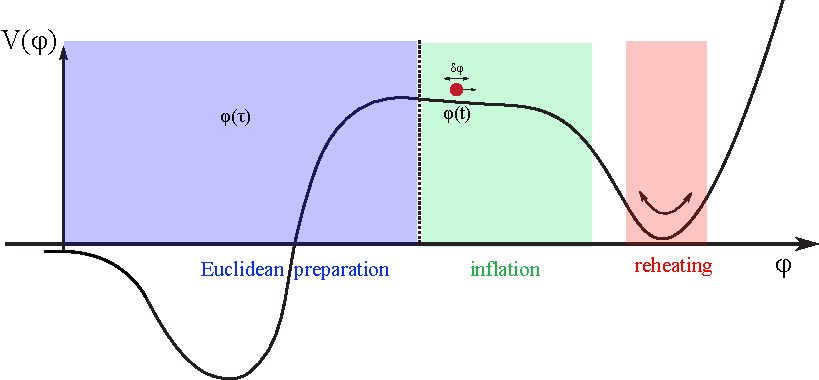
\includegraphics[width=0.6\linewidth]{Figures/PotentialHistory.pdf}
  \caption{Schematic representation of the desired potential that leads to inflationnary cosmology from a half-wineglass euclidean geometry. Figure from~\cite{betzios2024inflationarycosmologyantidesitter}. }
  \label{fig:potentialhistory}
\end{figure}
\subsection{Phase diagram of homogeneous and isotropic euclidean solutions in a concrete Einstein-Maxwell-dilaton model}
\begin{figure}[!h]
  \centering
  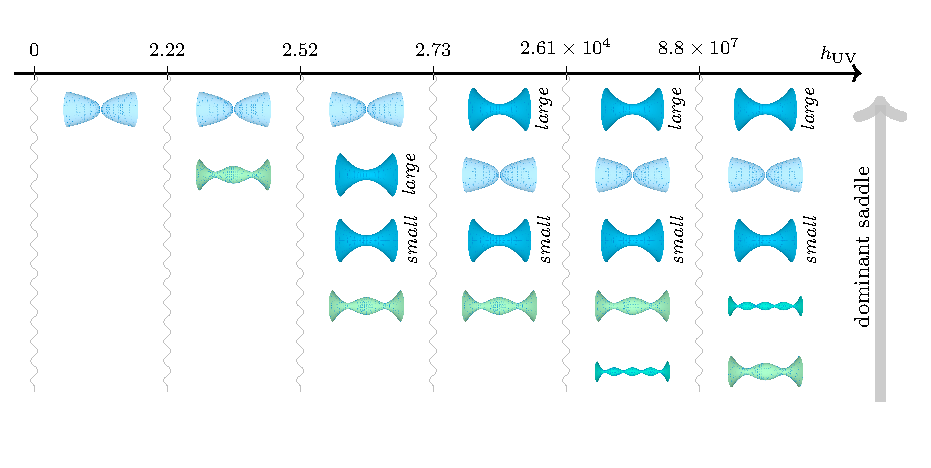
\includegraphics[width=0.8\linewidth]{Figures/Neumannphasediagram.pdf}
  \caption{Dominant saddles in the gravitational path integral across a range of $h_{\rm UV} \equiv (\k |\tilde{V}_{\rm AdS}|)^{1/2}H_{\rm UV}$. Some saddles cease to exist below certain minimum values $h_{\rm UV}^{\rm min}$. The labels \textit{large} and {\textit{small}} denote the two connected wormhole branches. Figure from~\cite{Betzios_2026}. }
  \label{fig:phasediagram_Neumannbdy}
\end{figure}
\subsection{Inclusion of perturbations}


\section{Updates of the current projects}
\subsection{Entanglement entropy in $c=1$ string theory}
\begin{figure}[!h]
  \centering
  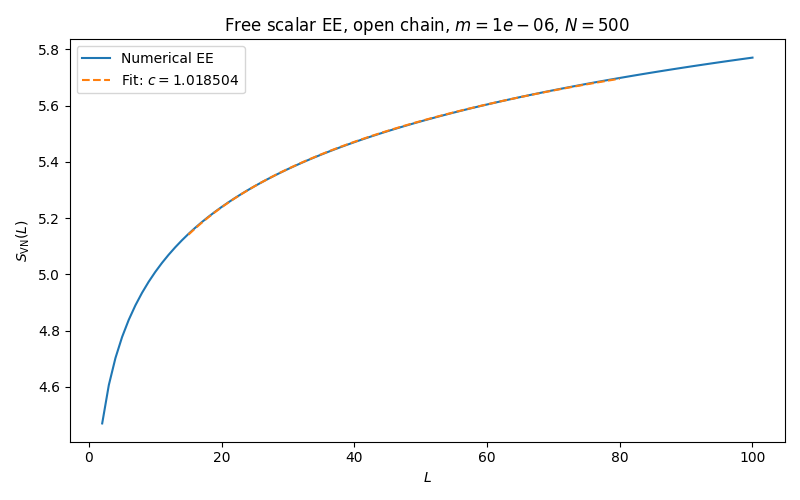
\includegraphics[width=0.6\linewidth]{Figures/open_freescalar.png}
  \caption{Fit of the entanglement entropy curve as a function of the size of the cut imposing open boundary conditions}
  \label{fig:open_freescalar}
\end{figure}

\begin{figure}[h!]
\centering
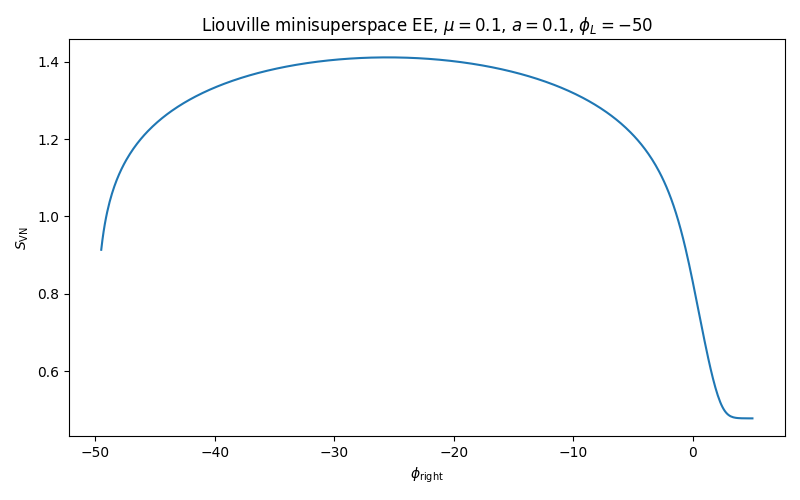
\includegraphics[width=0.72\textwidth]{Figures/entropybutleftrightnear.png}
\caption{Entanglement entropy as a function of the size of the cut imposing open boundary conditions for a detector crossing the horizon of a near extremal black hole.}
\label{fig:entropybutleftrightnear}
\end{figure}

\subsection{The bootstrap program of Timelike Liouville theory}
\subsection{Axion wormholes and Holography with the tools of dynamical system}

\begin{figure}[h!]
\centering
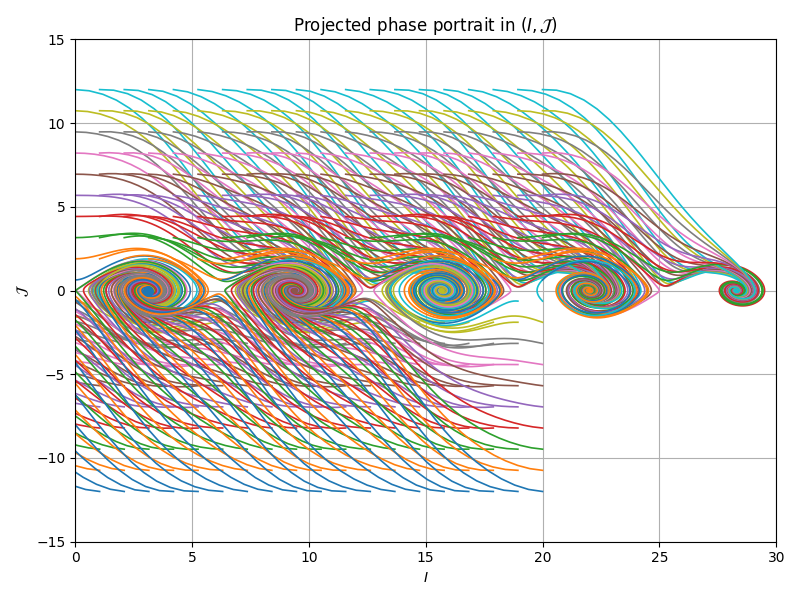
\includegraphics[width=0.72\textwidth]{Figures/phaseportraitv05alpha02d3.png}
\caption{Phase portrait with parameter $v_0=0.5,\,\alpha = 0.2,\,d=3$ and initial conditions $\mathcal{H}(0)=0$. $\sim400$ orbits are displayed.}
\label{fig:phaseportrait2}
\end{figure}

\begin{figure}[h!]
\centering
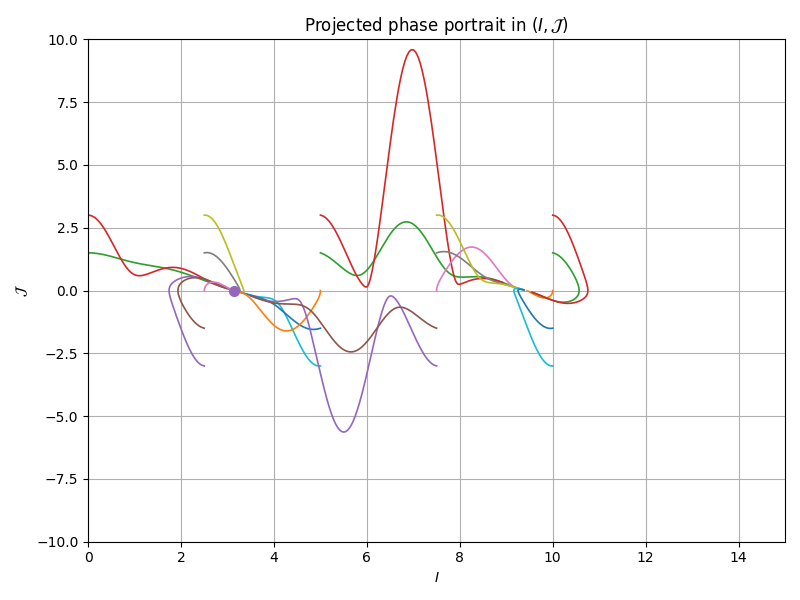
\includegraphics[width=0.72\textwidth]{Figures/phaseportraitv05alpha2d3.png}
\caption{Phase portrait with parameter $v_0=0.5,\,\alpha = 2,\,d=3$ and initial conditions $\mathcal{H}(0)=0$. $\sim30$ orbits are displayed.}
\label{fig:phaseportrait3}
\end{figure}

\subsection{Quantum effects of a Detector crossing the horizon of near extremal black hole}
\section{Conclusion}


\bibliographystyle{JHEP}
\bibliography{biblio}

\end{document}

